\chapter{Fresnel Simulation Toolbox}
\markboth{\MakeUppercase{Fresnel Simulation Toolbox}}{}
\label{chap:fresnel}
\section{Introduction}
\label{sec:intro}
This chapter describes a MATLAB simulation toolbox developed as a part of this doctorate project in order to investigate the potential of plenoptic imaging for biomedical and microscopy applications with particular interest in its behaviour at the diffraction limit. In literature are present many works on simulating plenoptic imaging devices. Plenoptic systems have been studied through simulation extensively. Until recently these studies have focussed on a geometrical optics approach, however in this project the focus is on investigating plenoptic systems biomedical and microscopy applications for which the performance at high resolution needs to be studied; hence diffraction cannot be ignored. Over the duration of this project there have been other research groups that have studied plenoptic systems under wave optics, including a wave optics analysis of plenoptic 1.0 systems, such as Schroff \textit{et al.} \cite{shroff2012high,shroff2013image} and Trujillo-Servilla \textit{et al.} \cite{birch2012depth} and a Fourier optics approach of the diffraction limit of a digital camera, Farrell \textit{et al.} \cite{farrell2012digital}. The growing interest in this aspect of plenoptic systems over the past few years is a product of the increasing interest in plenoptic systems overall and its new potential applications. In this work a Fresnel optics approach has been applied to a plenoptic camera with the purpose of understanding how the light field is recorded and to define some guidelines to design a working setup. Particular attention has been given to the behaviour of the system at its diffraction limit, a subject that has never been explicitly treated in literature. In this chapter four different methods to simulate light propagation in an optical system will be discussed and their performance compared in term of accuracy of the results, noise and computational effort.
A Fresnel optics approach has been chosen because the simulation tool to describe a plenoptic imaging system needs to have the following requirements:
\begin{itemize}
	\item it has to preserve the phase of the optical field propagating in order to preserve directional information of the rays of light;
	\item it has to take into account the effects of diffraction;
	\item it has to be adaptable in order to easily change the characteristic of the optical system, trying various configurations, keeping the operator based approach of ray tracing.
\end{itemize}
To address these features, a wave optics simulation toolbox has been designed and developed. Most of the existing literature on simulating plenoptic system are based on ray tracing techniques \cite{thurow2013recent,lynch2011development,lynch2012three,ng2006digital,levoy1996light}. The advantages of using ray tracing is that the transformations that rays undergo during the propagation can be described by two basic linear operators and compositions of them. These are the free space propagation and the lens operator. In developing the wave optics simulation this principle has been kept, and two operators have been defined: propagation and lens. Four different types of propagation operators have been described and compared. In analogy with ray tracing an optical system has been simulated using compositions of the two simple operators. In developing this platform all the media composing the system have been considered as linear, isotropic, homogeneous and non dispersive. 
\section{Scalar Theory of Diffraction}
\label{sec:scalar}
The term diffraction has been defined by Sommerfeld as any deviation of light rays from rectilinear paths which cannot be interpreted as reflection or refraction. \cite{sommerfeld1954optics}.The complex vectorial equations describing wave propagation in three dimensional space can be simplified into a set of scalar equations using the Scalar Theory of Diffraction as explained by Goodman \cite{goodman2005introduction}.
The starting point is given by Maxwell's Equations in absence of sources of electrical field of magnetic dipoles:\\
\begin{equation}
\label{eq:maxwell}
\begin{matrix}
	\nabla\times\overrightarrow{E}=-\mu\dfrac{\partial\overrightarrow{H}}{\partial t}\\
	\\
	\nabla\times\overrightarrow{H}=\epsilon\dfrac{\partial\overrightarrow{E}}{\partial t}\\
	\\
	\nabla\cdot\epsilon\overrightarrow{E}=0\\
	\\
	\nabla\cdot\mu\overrightarrow{H}=0\\
	\end{matrix}
\end{equation}
where $\overrightarrow{E}$ is the electric field, $\overrightarrow{H}$ is the magnetic field, $\mu$ and $\epsilon$ are respectively the magnetic permeability and electrical permittivity of the medium in which the optical wave is propagating. Both $\overrightarrow{E}$ and $\overrightarrow{H}$ are a functions of the position $x,y$ and $z$, as well as the time $t$. \\The operator $\nabla$ is defined as:\\
\begin{equation}
\label{eq:nabla}
	\nabla=\dfrac{\partial}{\partial x}\widehat{i}+\dfrac{\partial}{\partial y}\widehat{j}+\dfrac{\partial}{\partial z}\widehat{k}
\end{equation}
where $\widehat{i},\widehat{j}$ and $\widehat{k}$ are unit vectors along directions $x,y$ and $z$.\\
Propagation is assumed to happen in a dielectric medium that is linear, isotropic and homogeneous. A medium is linear if its response to a several disturbances acting simultaneously can be decomposed into the sum of the responses to the single disturbances taken individually. It is isotropic if its properties do not depends on the directions of polarization of the wave and is homogeneous if its permittivity is constant along all direction of propagation. The medium is considered also to be non dispersive, that is the permittivity $\epsilon$ is not dependent on the wavelength. \\
Applying the operator $\nabla\times$ to the left and to the right side of the first equation of \ref{eq:maxwell} and using the vector identity\\
\begin{equation}
\label{eq:vectidentity}
\nabla\times(\nabla\times\overrightarrow{E})=\nabla (\nabla\cdot\overrightarrow{E})-\nabla^2\overrightarrow{E}
\end{equation}
\begin{equation}
\label{eq:wave1}
	\nabla (\nabla\cdot\overrightarrow{E})-\nabla^2\overrightarrow{E}=\nabla\times(-\mu\dfrac{\partial\overrightarrow{H}}{\partial t})\\
\end{equation}
From the third equation in \ref{eq:maxwell}:\\
\begin{equation}
\label{eq:divergenza}
\nabla\cdot\epsilon\overrightarrow{E}=0\\
\end{equation}
hence equation \ref{eq:wave1} becomes:\\
\begin{equation}
\label{eq:wave2}
-\nabla^2\overrightarrow{E}=\nabla\times(-\mu\dfrac{\partial\overrightarrow{H}}{\partial t})\\
\end{equation}
since both the operators $\nabla\times$ and its derivative are linear it is possible to swap them on the right hand side of equation \ref{eq:wave1}.
Then substituting the second Maxwell equation \ref{eq:maxwell} into the equation \ref{eq:wave2}:
\begin{equation}
\label{eq:wave3}
-\nabla^2\overrightarrow{E}=-\mu\epsilon\dfrac{\partial^2}{\partial t^2}\overrightarrow{E}	
\end{equation}
Where $\nabla^2$ is the Laplacian operator defined as:
\begin{equation}
	\label{eq:laplacian}
	\nabla^2=\dfrac{\partial^2}{\partial x^2}\widehat{i}+\dfrac{\partial^2}{\partial y^2}\widehat{j}+\dfrac{\partial^2}{\partial z^2}\widehat{k}	
\end{equation}
The refractive index of the medium in which the wave is propagating is:\\
\begin{equation}
\label{eq:n}
n=\sqrt{\dfrac{\epsilon\mu}{\epsilon_0\mu_0}}
\end{equation} 
where $\epsilon_0$ is the permittivity of the vacuum and $\mu_0$ the magnetic permeability in vacuum. Therefore the speed of light in the vacuum is:
\begin{equation}
\label{eq:speedoflight}
c=\sqrt{\dfrac{1}{\epsilon_0\mu_0}}
\end{equation} 
Then the wave equation for the electric field becomes:
\begin{equation}
\label{eq:wave_elec}
\nabla^2\overrightarrow{E}-\dfrac{n^2}{c^2}\dfrac{\partial^2\overrightarrow{E}}{\partial t^2}=0
\end{equation}
Similar considerations can be done for the magnetic field, leading to an identical equation:
\begin{equation}
\label{eq:wave_magn}
\nabla^2\overrightarrow{H}-\dfrac{n^2}{c^2}\dfrac{\partial^2\overrightarrow{H}}{\partial t^2}=0
\end{equation}
Since the wave equation is obeyed by both the electric field and magnetic fields, it is possible to define a scalar wave equation, obeyed by the single components of those vectors. The scalar field components are represented as a function $u(x,y,z,t)$ called field disturbance.
The scalar wave equation is then:
\begin{equation}
\label{eq:scalar_wave}
\nabla^2u-\dfrac{n^2}{c^2}\dfrac{\partial^2u}{\partial t^2}=0
\end{equation}
With this scalar approximation it is possible to treat the propagation of an optical field as a scalar. This is only valid under the assumption of a linear, isotropic, homogeneous and non dispersive medium, since all the component in all the directions of the electric and magnetic fields must behave identically.
\subsection{Helmholtz Equation}
In the case of monochromatic waves the scalar field $u$ is a function of time $t$ and position $\overrightarrow{X}$ defined as:
\begin{equation}
\label{eq:scalarfield}
u(\overrightarrow{X},t)=A(\overrightarrow{X})cos[2\pi\nu t-\phi(\overrightarrow{X})]
\end{equation}
Where $A(\overrightarrow{X})$ is the amplitude of the disturbance and $\phi(\overrightarrow{X})$ is its phase at a point in the space with coordinates $\overrightarrow{X}=(x,y,z)$.
Separating space and time dependence:
\begin{equation}
\label{eq:scalarfield2}
u(\overrightarrow{X},t)=Re\{{U(\overrightarrow{X})e^{-j2\pi\nu t}}\}
\end{equation}
where $U$ is a complex function of position and includes the phase term $e^{j\phi(\overrightarrow{X})}$.
\begin{equation}
\label{eq:scalarfield3}
U(\overrightarrow{X})=A(\overrightarrow{X})e^{j\phi(\overrightarrow{X})}
\end{equation}
This field should satisfy the scalar wave equation \ref{eq:scalar_wave}. Substituting equation \ref{eq:scalarfield3} into \ref{eq:scalar_wave}:
\begin{equation}
\label{eq:scalar1}
	\nabla^2[U(\overrightarrow{X})e^{-j2\pi\nu t}]-\dfrac{n^2}{c^2}\dfrac{\partial^2}{\partial t^2}[U(\overrightarrow{X})e^{-j2\pi\nu t}]=0
\end{equation}
Expressing the derivatives and simplifying the exponential terms:
\begin{equation}
\label{eq:scalar2}
\nabla^2[U(\overrightarrow{X})]+ \left(\dfrac{2\pi\nu n}{c}\right)^2[U(\overrightarrow{X})]=0
\end{equation}
The wave number is defined as:
\begin{equation}
\label{eq:wavenumber}
	k=\dfrac{2\pi\nu n}{c}
\end{equation}
and expression \ref{eq:scalar2} becomes:
\begin{equation}
\label{eq:helmotz}
(\nabla^2+k^2)U=0	
\end{equation}
Equation \ref{eq:helmotz} is the Helmholtz equation and it describes the behaviour of a complex disturbance propagating in a homogeneous medium.
\subsection{Solutions of Helmholtz Equations}
 An analytical expression of the complex disturbance $U$ that satisfies the Helmholtz equation can be found using the Green's theorem under particular boundary conditions as explained by Goodman \cite{goodman2005introduction}. There are two possible solutions: Fresnel-Kirchhoff and Rayleigh-Sommerfeld.
Considering a wave $U_0$ propagating through a diffracting screen at a point in space with coordinates $z=0$ with an aperture $D$ the boundaries conditions:
\begin{itemize}
	\item Fresnel-Kirchhoff (FK) conditions \\
	\begin{math}
		\label{eq:FKbound}
		U(x,y;0)=U_0(x,y;0) \quad for \quad (x,y)\in D\\
		U(x,y;0)=0 \quad for \quad (x,y)\notin D\\
		\\
		\dfrac{\partial U}{\partial z}=\dfrac{\partial U_0}{\partial z} \quad for \quad (x,y)\in D\\
		\\
		\dfrac{\partial U}{\partial z}=0 \quad for \quad (x,y)\notin D\\	
		\end{math}
	\item Rayleigh-Sommerfeld (RS) conditions:\\
	\begin{math}
	U(x,y;0)=U_0(x,y;0) \quad for \quad (x,y)\in D\\
	U(x,y;0)=0 \quad for \quad (x,y)\notin D\\
	\end{math}
\end{itemize}
	The FK conditions lead to a simple result but they are not physically correct since they imply the field after the screen to be zero outside of the aperture in the immediate proximity of the screen as well as its normal derivative. Results given by the FK condition are accurate only for a distance from the aperture much larger than the wavelength.
	The RS condition on the other hand is less strict since it does not requires the derivatives of the disturbance and leads to a solution of the Helmholtz equation that is:
	\begin{equation}
	\label{eq:RSintegral}
	U(x,y;z)=\dfrac{1}{j\lambda}\iint_{\sigma}^{}U(\xi,\eta;0)\dfrac{e^{jkr}}{r} \cos(\theta) d\xi d\eta
		\end{equation}
		where, with reference to figure \ref{fig:RS}, $\theta$ is the angle between the z axis and the direction of propagation, $r=\sqrt{z^2+(x-\xi)^2+(y-\eta)^2}$ is the distance between the point $P_1=(x,y,z)$ and $P_0=(\xi,\eta;0)$ and $\sigma$ is the area of aperture. Since $\cos(\theta)=\dfrac{z}{r}$:
		\begin{equation}
		\label{eq:RSintegral1}
		U(x,y;z)=\dfrac{z}{j\lambda}\int\int_{\sigma}^{}U(\xi,\eta;0)\dfrac{e^{jkr}}{r^2} d\xi d\eta
		\end{equation}
		Equation \ref{eq:RSintegral1} is the Rayleigh-Sommerfeld diffraction formula \cite{goodman2005introduction}, and can be simplified under the Fresnel approximation, as will be explained in section \ref{sec:fresnelapprox}.
		\begin{figure}[H]
			\begin{center}
				\begin{tabular}{c}
					\includegraphics[height=5cm]{RS.eps}
				\end{tabular}
			\end{center}
			\caption{ \label{fig:RS} 
				Geometry of the aperture. }
		\end{figure} 
\subsection{The Fresnel Approximation}
\label{sec:fresnelapprox}
It is possible to approximate the distance of propagation $r$ between $P_0$ and $P_1$ with its Taylor expansion up to the second order:
\begin{equation}
\label{eq:taylor}
r=\sqrt{1+\left(\dfrac{x-\xi}{z}\right)^2+\left(\dfrac{y-\eta}{z}\right)^2}\approx z\left[1+\frac{(1)}{2}\left(\dfrac{x-\xi}{z}\right)^2+\frac{1}{2}\left(\dfrac{y-\eta}{z}\right)^2\right]
\end{equation}
Therefore for large propagation distances, $z\gg x,y$, the diffraction integral becomes:
\begin{equation}
\label{eq:Fresnel}
	U(x,y)=\dfrac{e^{jkz}}{j\lambda z} \int\int_{-\infty}^{\infty}U(\xi,\eta)e^{\frac{jk}{2z}\left[(x-\xi)^2+(y-\eta)^2\right]} d\xi d\eta
\end{equation}
Factorizing the exponential term the disturbance becomes:
\begin{equation}
\label{eq:Fresnel1}
U(x,y)=\dfrac{e^{jkz}}{j\lambda z} e^{j\frac{k}{2z}(x^2+y^2)} \int\int_{-\infty}^{\infty}U(\xi,\eta)e^{\frac{jk}{2z}(\xi^2+\eta^2)}e^{\frac{-jk}{2z}(x\xi+y\eta)} d\xi d\eta
\end{equation}
This can be seen as the Fourier transform of the disturbance before the aperture $U(\xi,\eta)$ multiplied by a quadratic phase factor
 $e^{\frac{jk}{2z}(\xi^2+\eta^2)}$ \cite{goodman2005introduction}.
\section{Free Space Propagation Operator: Fresnel Approximation Approach}
\label{sec:Fresnel}
The first version of the free space propagation operator has been developed using the Fresnel Integral as written in equation \ref{eq:Fresnel1}.
The input disturbance $U(\xi,\eta)$ is considered to be illuminated by monochromatic light with wavelength $\lambda$. As stated in section \ref{sec:fresnelapprox} the Fresnel integral can be seen as the two dimensional Fourier transform of the input field $U(\xi,\eta)$ multiplied by a quadratic phase factor \cite{goodman2005introduction, sypek1995light}. This is going to be very useful from a computational point of view since it can be implemented with a fast The function $U'(\xi,\eta)$ is defined as:
\begin{equation}
	\label{eq:U1}
	U'(\xi,\eta)=U(\xi,\eta)e^{\frac{jk}{2z}(\xi^2+\eta^2)}
\end{equation}
The optical field at the plane $z$ is the product of the Fourier transform of $U'(\xi,\eta)$ with the phase term $e^{\frac{jk}{2z}(x^2+y^2)}$:
\begin{equation}
	\label{eq:FT1}
	U(x,y) = \dfrac{e^{ikz}}{i\lambda z}e^{\frac{ik}{2z}(x^2+y^2)}\mathcal{F}[U'(\xi,\eta)]
\end{equation}
where the spatial frequencies of the Fourier Transform can be correlated with the spatial coordinates $x$ and $y$ by the relation:
\begin{equation}
\label{eq:spacefreq}
\left\{
\begin{array}{l l}
 f_x=\frac{x}{\lambda z} \\
 f_y=\frac{y}{\lambda z}
\end{array} \right.\
\end{equation}
This method is computationally fast since it requires only one Fourier transform, and it is analytically correct. Particular attention should be given to the sampling of the optical fields U and U'. Because of the presence of the Fourier transform the coordinates of the input and output fields are not sampled in the same way, but are scaled by a factor that is proportional to the distance of propagation, as shown in equation \ref{eq:spacefreq} \cite{gonzalez2004digital}. Therefore the input and output planes have different sampling \cite{sypek1995light}.
In addition the multiplicative phase factor:
\begin{equation}
\label{eq:phase2}
e^{\frac{ik}{2z}(\xi^2+\eta^2)}
\end{equation}
presents rapid oscillation of the phase of the optical field for small variations of z, since z is at its denominator \cite{sypek1995light, matsushima2009band}. In order to avoid aliasing the input field requires a large sampling and this is achieved by zero padding the sampling window of the input field, with an increase of the digital resolution of the field. It is known that the computational effort of the FFT algorithm increases with the resolution as $O(n \log n)$, where $n$ is the number of samples of the input field and increasing the sampling resolution of the field \cite{bracewell1965fourier} leads to a long computational time. 
\subsection{Multi-Step Fresnel Propagation Operator}
\label{sec:fresnelmulti}
To overcome the scaling of the field and the large computational time required by the Fresnel propagation integral method a modified method has been developed. 
A multi step approach as the one explained by Sypek \cite{sypek1995light, sypek2009reply} and shown in figure \ref{fig:multistepfig} was used. 
\begin{figure}[h]
	\begin{center}
		\begin{tabular}{c}
				\includegraphics[height=6cm]{multistepfig.eps}
		\end{tabular}
	\end{center}
	\caption{\label{fig:multistepfig} To remove the scaling factor between the input and output fields, a multi step Fresnel approach has been developed. The field is propagated by unit of dz, the minimum distance to keep the sampling the same. } 
	\end{figure}
The reason to adopt the multi-step approach in this project is to remove the scaling factor between the input field and the output field that arise from the Fourier transform as shown in equation \ref{eq:spacefreq}, while Sypek developed a multi step propagation model to minimize the oscillations of the Fourier spectrum and to avoid large zero paddings.\\ In the Fourier domain, an optical field sampled by a $N \times N$ pixels window, and with squared pixels that are $dx$ wide the spatial frequency resolution is \cite{bracewell1965fourier,gonzalez2004digital}:
\begin{equation}
\label{eq:getz1}
df_x=\dfrac{1}{Ndx}
\end{equation}
 Therefore the pixel size in the image plane is according to equations \ref{eq:spacefreq}:
\begin{equation}
\label{eq:pixelsize}
d\xi=d\nu\lambda z
\end{equation} 
where $z$ is the propagation distance and $\lambda$ is the wavelength of the monochromatic wave. The condition to keep the same resolution both in the input field and the output field is:
\begin{equation}
\label{eq:getz}
d\xi=df_x\lambda z=dx
\end{equation}
Substituting equation \ref{eq:getz1} into equation \ref{eq:spacefreq}:
\begin{equation}
\label{eq:getz2}
\dfrac{1}{Ndx}=\frac{dx}{\lambda z}
\end{equation}
Then resolving for z the minimum propagation distance $dz$ to keep the same sampling both in the input and output fields is:
\begin{equation}
\label{eq:getz3}
dz=\frac{W^2}{N\lambda }
\end{equation}
and:
\begin{equation}
	\label{eq:getz4}
	z=\displaystyle\sum_{i=1}^{N} dz_i
\end{equation}
where $W=Ndx$ is the dimension in meters of the input field. Equation \ref{eq:getz3} gives the length of the single step in which the propagation distance $z$ should be divided in order to keep the same resolution.\\ Although the results obtained with this multi-step approach are correct there are some issues. The propagation distance should be a multiple of $dz $, and this is a very significant limitation, especially since in simulating plenoptic systems the distances need to be set precisely. Another issue regards the computational time. With the multi step approach the number of FFT performed increases with the steps, leading to a computational time \textit{N} times larger that the Fresnel Integral method. For these reasons the angular spectrum method as will be discussed in section \ref{sec:angular} has been adopted in all the simulations presented in this work. 
\section {Free Space Propagation Operator: Angular Spectrum of Plane Waves Approach}
\label{sec:angular}
 In the Fourier domain the input disturbance can be seen as formed by a set of plane waves travelling in different directions, the \textit{Angular Spectrum of Plane waves} representation of an optical field. In the next section the propagation operator as and its characteristic transfer function will be defined. Three versions of the angular spectrum operator will be presented, and performances of the three versions will be compared.
\subsection{Angular Spectrum of Plane Waves}
\label{sec:angular 2}
The disturbance $U(x,y;0)$ describing a monochromatic wave incident on a plane \textit{(x,y)} at the \textit{z=0} while travelling along the z direction has a Fourier transform given by:
\begin{equation}
\label{eq:AS1}
A(f_x,f_y;0)=\iint_{-\infty}^{\infty} U(x,y;0)e^{-j2\pi(f_x x+f_y y)}dx dy
\end{equation}
and $U(x,y;0)$ is equal to the inverse Fourier transform of its spectrum:
\begin{equation}
\label{eq:AS2}
U(x,y;0)=\iint_{-\infty}^{\infty} A(f_x,f_y;0)e^{j2\pi(f_x x+f_y y)}df_x df_y
\end{equation}
The physical meaning fo the equation \ref{eq:AS2} is that the disturbance $U(x,y;0)$ can be decomposed in the sum of elemental plane waves propagating in directions given by the wave vector $\overrightarrow{k}$ whose magnitude is $2\pi/\lambda$ and direction is given by its direction cosines $(\alpha,\beta,\gamma)$ \cite{goodman2005introduction,matsushima2009band}.
Dropping the temporal dependence the plane wave is then:
\begin{equation}
\label{eq:AS3}
p(x,y;z)=e^{-j\overrightarrow{k}\cdot\overrightarrow{r}}\\
\end{equation}
where
\begin{equation}
\label{eq:AS4}
 \overrightarrow{r}=x\widehat{i}+y\widehat{j}+z\widehat{k}\\
\end{equation}
and
\begin{equation}
\label{eq:AS5}
 \overrightarrow{k}=\dfrac{2\pi}{\lambda}(\alpha\widehat{i}+\beta\widehat{j}+\gamma\widehat{k})	\\
\end{equation}
The exponential becomes:
\begin{equation}
\label{eq:AS6}
p(x,y;z)=e^{-j\frac{2\pi}{\lambda}(\alpha x+\beta y)}e^{-j\frac{2\pi}{\lambda}(\gamma z)}
\end{equation}
The terms, $\alpha, \beta$ and $\gamma$ are the direction cosines of the wave vector $\overrightarrow{k}$ and they are related as:
\begin{equation}
\label{eq:AS7}
\gamma = \sqrt{1-\alpha^2+\beta^2}
\end{equation}
Therefore the complex exponential function in equation \ref{eq:AS1} can be seen as a plane wave with direction cosines
\begin{equation}
\label{eq:AS8}
\alpha=\lambda f_x, \ \ \beta=\lambda f_y, \ \ \gamma = \sqrt{1-(\lambda f_x)^2+(\lambda f_y)^2}
\end{equation}
The angular spectrum of plane waves of the disturbance $U(x,y;0)$ is the function:
\begin{equation}
\label{eq:AS9}
A\left(\frac{\alpha}{\lambda},\frac{\beta}{\lambda};0\right)=\iint_{-\infty}^{\infty} U(x,y;0)e^{-j2\pi(\frac{\alpha}{\lambda} x+\frac{\beta}{\lambda} y)}dx dy
\end{equation}
After a prorogation of $z$ the disturbance $U(x,y;z)$ can be written in the form of the angular spectrum in analogy with equation \ref{eq:AS2}:
\begin{equation}
\label{eq:AS10}
U(x,y;z)=\iint_{-\infty}^{\infty} A(f_x,f_y;z)e^{j2\pi(f_x x+f_y y)}df_x df_y
\end{equation}
where $f_x=\alpha/\lambda$ and $f_y=\beta/\lambda$.
To be a propagative disturbance, equation \ref{eq:AS10} should satisfy the Helmholtz equation \ref{eq:helmotz}:
\begin{equation}
\label{eq:AS11}
(\nabla^2+k^2)U=0	
\end{equation}
Substituting equation \ref{eq:AS10} into \ref{eq:AS11}:
 \begin{equation}
 \label{eq:AS12}
\dfrac{d^2}{dz^2}A(f_x,f_y;z)+\left(\dfrac{2\pi}{\lambda}\right)[1-(\lambda f_x)^2 + (\lambda f_y)^2 ]A(f_x,f_y;z)=0
 \end{equation}
 A solution of the differential equation \ref{eq:AS12} is:
 \begin{equation}
 \label{eq:AS13}
 A(f_x,f_y;z)=A(f_x,f_y;0)e^{j \frac{2\pi}{\lambda}\sqrt{1-(\lambda f_x)^2+(\lambda f_y)^2}}
 \end{equation}
 The propagative solution is the one where the spatial frequencies satisfy the condition:
 \begin{equation}
 \label{eq:AS14}
 (\lambda f_x)^2+(\lambda f_y)^2<1
 \end{equation}
 in this case the exponential term in equation \ref{eq:AS13} remains complex and the wave can propagate since it is an oscillating term. For the values of spatial frequencies that satisfy the condition:
 \begin{equation}
 \label{eq:AS15}
 (\lambda f_x)^2+(\lambda f_y)^2>1
 \end{equation}
 the exponent in the equation \ref{eq:AS13} becomes real, and the exponential is a decay term. The solution is no longer propagative and waves are called evanescent waves. It is interesting to see how the angular spectrum theory is more complete than the Fresnel approximation since it includes evanescent components too.\\
 Finally, the disturbance after a propagation in z can be expressed as a function of the disturbance $U(x,y;0)$ at the plane z=0:
 \begin{equation}
 \label{eq:AS16}
 U(x,y;z)=\int\int_{-\infty}^{\infty} A(f_x,f_y;0)e^{j \frac{2\pi}{\lambda}\sqrt{1-(\lambda f_x)^2-(\lambda f_y)^2}}e^{j2\pi(f_x x+f_y y)}df_x df_y
 \end{equation}
 The last equation enables a calculation of the output field $U(x,y;z)$ in terms of the input field and the propagation distance, under the approximation of a linear, isotropic, homogeneous and non dispersive medium.\\
 Because of the linearity of the problem, the propagation is considered as a linear system that maps the input disturbance $U(x,y;0)$ into the a new field distribution $U(x,y;z)$\cite{goodman2005introduction}. This linear system is characterized by a transfer function whose bandwidth is limited to the case of the propagative solution of equation \ref{eq:AS12}, excluding the evanescent waves. The angular spectrum of the output field can be rewritten as the product of the angular spectrum of the input field multiplied by the transfer function $H(f_x,f_y)$:
 \begin{equation}
 \label{eq:AS17}
 A(f_x,f_y;z) = A(f_x,f_y;0)\cdot H(f_x,f_y;z)
 \end{equation}
 The propagation is fully described by the transfer function:
 \begin{equation}
 \label{eq:AS18}
H(f_x,f_y;z)=\begin{cases}e^{j \frac{2\pi z}{\lambda}\sqrt{1-(\lambda f_x)^2-(\lambda f_y)^2}} & \quad \text{if } \sqrt{f_x^2+f_y^2}<\frac{1}{\lambda}\\ 0 & \quad \text{otherwise }\\ \end{cases} 
 \end{equation}
 The bandwidth can be represented as a circle in Fourier space. For frequencies smaller than $1/\lambda$ the transfer function introduces a shift in the spatial domain that is responsible for diffraction \cite{goodman2005introduction}.
 Results obtained with the angular spectrum method are similar to the ones obtained with the Fresnel approximation, but no scaling factor between the input and output field is introduced. 
 From a computational point of view, the angular spectrum operator is composed of 3 steps: 
 \begin{enumerate}
 	\item Fourier transform of the input field
 	\item Multiplication of the Fourier transform of the input field with the propagation transfer function in equation \ref{eq:AS18} 
 	\item Inverse Fourier transform of the product at step 2. The resultant field is the output disturbance after the propagation in free space. 
 \end{enumerate}
 The process can be seen in figure \ref{fig:ASflux}
 \begin{figure}[H]
 	\begin{center}
 		\begin{tabular}{c}
 				\includegraphics[height=1.5cm]{asflux.eps}
 				\end{tabular}
 		\end{center}
 			\caption{ \label{fig:ASflux} 
 				Structure of the operator free space propagation with the angular spectrum of plane waves method. The initial disturbance $U(x,y;0)$ is transformed into the angular spectrum $A(f_x,f_y;0)$ with a Fourier transform implemented by a FFT algorithm. The angular spectrum is multiplied by the propagation transfer function $H(f_x,f_y)$ and the resultant angular spectrum is inverse transformed into the output disturbance $U(x,y;z)$ }
 \end{figure}
 \subsection{Band Limited Angular Spectrum}
 The transfer function of the propagation in equation \ref{eq:AS18} is a complex exponential oscillating with a frequency depending by the propagation distance $z$. Figure \ref{fig:AStransfer} shows four different profiles of the transfer function for four propagation distances, \textit{1 mm, 2 mm, 10 mm and 20 mm}. Aliasing effects are evident since for a propagation distance of \textit{2 mm}. When the \textit{z} becomes large, the aliasing arises at low spatial frequencies, narrowing the useful bandwidth of the transfer function \cite{matsushima2009band}.
 The transfer function can be rewritten as:
 \begin{equation}
 	\label{eq:BL1}
 	H(f_x,f_y) = e^{j \phi(f_x,f_y)}
 \end{equation}
 where $\phi$ is the oscillating phase term as:
 \begin{equation}
 	\label{eq:BL2}
 	\phi(f_x,f_y)=\dfrac{2\pi}{\lambda}\sqrt{1-\lambda f_x^2-\lambda f_y^2}
 \end{equation}
 \newpage
 \begin{figure}[H]
 	\begin{center}
 		\begin{tabular}{c}
 			\includegraphics[height=16cm]{phaseH01.eps}
 		\end{tabular}
 	\end{center}
 	\caption 	{ \label{fig:AStransfer} 
 		Cross section along of the phase of the transfer function of the angular spectrum. It is evident how increasing the propagation distance increases the oscillating frequency leading to aliasing. }
 \end{figure}
 \newpage
 Defining the local spatial frequencies of the transfer function \cite{goodman2005introduction,matsushima2009band} as the frequency of the phase oscillation $\nu_x$ and $\nu_y$ along $f_x$ and $f_y$:
 \begin{equation}
 	\label{eq:BL3}
 	\begin{cases} \nu_x=\dfrac{1}{2\pi}\dfrac{\partial}{\partial f_x}\phi(f_x,f_y)\\
 	\\
 	 \nu_y=\dfrac{1}{2\pi}\dfrac{\partial}{\partial f_y}\phi(f_x,f_y)\\ \end{cases}
 \end{equation}
 the local spatial frequencies become:
 \begin{equation}
 \label{eq:BL16}
 \begin{cases} \nu_x=-\dfrac{z}{\lambda}\dfrac{\lambda^2 f_x}{\sqrt{1-(\lambda f_x)^2}}\\
 \\
 \nu_y=-\dfrac{z}{\lambda}\dfrac{\lambda^2 f_y}{\sqrt{1-(\lambda f_y)^2}}\\ \end{cases}
 \end{equation}
 As stated by Matsushima and Shimobaba \cite{matsushima2009band}, if the input optical disturbance is sampled by an $N \times N$ sampling window with pixel size $dx$, the transfer function is sampled by units of spatial frequency equal to $df=1/(N dx)$. To satisfy the Nyquist condition the sampling frequency should be at least the double of the bandwidth of the transfer function. For one direction in the local frequency space:
 \begin{equation}
 \label{eq:BL4}
 \dfrac{1}{df}\geq 2|\nu_x|
 \end{equation}
 Modifying the sampling of the transfer function, and of the input field, can lead to huge sampling windows and long computational times. In addition to that in practical applications the sampling interval is usually fixed. Therefore the condition on the maximum frequency range for which the transfer function is not aliased:
 \begin{equation}
 \label{eq:BL5}
 \dfrac{1}{df_x}\geq 2 z\dfrac{|f_x|}{|\sqrt{(\frac{1}{\lambda^2}+f_x)^2}|}\\ 
 \end{equation}
 Resolving the equation for $|f_x|$ :
 \begin{equation}
 \label{eq:BL6}
 |f_x|\leq\dfrac{1}{\lambda\sqrt{(2df_x z)^2+1}} = f_{max}
 \end{equation}
 Where $f_{max}$ is the maximum frequency of the transfer function without generating errors due to aliasing. Assuming the sampling of the optical field to be the same in both x and y direction the maximum bandwidth for the sampling in $f_y$ is equal to the bandwidth in $f_x $. Therefore:
 \begin{equation}
 \label{eq:BL7}
 \dfrac{1}{df_y}\geq 2|\nu_y|
 \end{equation}
 \begin{equation}
 \label{eq:BL8}
 \dfrac{1}{df_y}\geq 2 z\dfrac{|f_y|}{|\sqrt{(\frac{1}{\lambda^2}+f_y)^2}|}\\ 
 \end{equation}
 \begin{equation}
 \label{eq:BL9}
 |f_y|\leq\dfrac{1}{\lambda\sqrt{(2df_y z)^2+1}} = f_{max}
 \end{equation}
 To avoid aliasing then, the two dimensional transfer function should be limited to a range of frequencies defined by equation \ref{eq:BL8}.
 The expression of the output field will then be:
 \begin{equation}
 \label{eq:BL10}
 U(x,y;z)= \mathcal{F}^{-1}\left[A(f_x,f_y;0)H'(f_x,f_y;z)\right]
 \end{equation}
 where
 \begin{equation}
 \label{eq:BL11}
 H'(f_x,f_y;z)=H(f_x,f_y;z)rect\left(\dfrac{f_x}{f_{max}}\right)rect\left(\dfrac{f_y}{f_{max}}\right)
 \end{equation}
 The MATLAB algorithm to implement the band limitation consists in multiplying the phase term of the propagation transfer function by a phase mask with the shape of a circle function of radius $f_{max}$ in the plane of the spatial frequencies. A circular phase mask has been chosen instead of the rectangular phase mask of equation \ref{eq:BL11} because it follows the geometry of the lens aperture, without introducing new spatial features that could effect the diffraction.\\ The resultant phase of the transfer function is shown in figure \ref{fig:bandlimitedH}, with the bandwidth for three different propagation distances.
 \begin{figure}[H]
 	\begin{center}
 		\begin{tabular}{c}
 				\includegraphics[height=15cm]{phaseHBL.eps}
 		\end{tabular}
 	\end{center}
 	\caption { \label{fig:bandlimitedH} 
 		Bandwidth of the transfer function for three different propagation distances. }
 \end{figure} 
 From a computational point of view the algorithm to implement the band limited angular spectrum method can be summarized in the following steps:
 \begin{enumerate}
		\item Computation of the angular spectrum of the input disturbance via a Fourier transform as shown in equation \ref{eq:AS2}.
		\item Estimation of the maximum bandwidth of the transfer function in order to avoid aliasing error using equation \ref{eq:BL6}.
		\item Multiplication of the phase of the transfer function with a circular phase mask with radius equal to the frequency obtained in the previous step.
		\item Multiplication of the angular spectrum with the band limited transfer function.
		\item Inverse Fourier transform of the product at step 4 
 \end{enumerate}
 The structure of the free space propagation operator implemented by the band limited angular spectrum can be seen in figure \ref{fig:BLAS} 
 \newpage
 \begin{figure}[H]
 	\begin{center}
 		\begin{tabular}{c}
 			\includegraphics[height=5cm]{asfluxBL.eps}
 		\end{tabular}
 	\end{center}
 	\caption	{ \label{fig:BLAS} 
 		Structure of the operator free space propagation with the angular spectrum of plane waves method in its band limited version. The initial disturbance $U(x,y;0)$ is transformed into the angular spectrum $A(f_x,f_y;0)$ with a Fourier transform implemented by a FFT algorithm. The angular spectrum is multiplied by the propagation transfer function $H(f_x,f_y)$ whose bandwidth has been limited according to equation \ref{eq:BL9}. The bandwidth of the transfer function depends on the sampling of the input field, the wavelength of the light $\lambda$ and the propagation distance.The resultant angular spectrum is inverse transformed into the output disturbance $U(x,y;z)$. \textit{N} is the sampling of thr input field, \textit{z} the propagation distance and $\lambda$ the wavelength. }
 \end{figure} 
 \subsection{Corrected Band Limited Angular Spectrum Method}
 \label{sec:angular3}
 The third method to implement the propagation operator with the angular spectrum is the corrected band limited angular spectrum method. The difference between this method and the band limited angular spectrum method presented in section \ref{sec:angular 2} is that the bandwidth of the transfer function is truncated to the value of the cut-off frequency of the free space propagation in case the Nyquist criterion requires a bandwidth is too narrow.\\
 For long propagation distances the propagation transfer function acts as a low pass filter on the spatial frequency components of the input signal. When its bandwidth is bigger than the cutoff frequency calculated with the band limited method to avoid digital aliasing there is a loss of resolution in the final image. A trade-off should therefore be found between the error due to the aliasing and the error due to the excessive bandwidth limitation. For imaging applications this is not an issue since usually the numerical apertures of the optical elements in the imaging system already limit the band passing from the input field to the output field. However it is useful to estimate the bandwidth of the free space propagation defining the maximum spatial frequency that is transferred from the object plane to the image plane. This value defines the amount of information transferred from the input field to the image plane.\\
 With reference to figure \ref{fig:maxfrequency} for a point in the input field, the range of spatial frequencies that are transferred to the output field are the ones whose direction cosines are contained into the angle that includes the sampling window of the output field. In the cases of the propagation distance much bigger than the sampling window, $z>>W $ like in most of the applications of this simulation toolbox the angle $\theta$ is equal to:
 \begin{equation}
 \label{eq:BL12}
 \theta \simeq\dfrac{W}{z}
 \end{equation}
 \begin{figure}[h]
 	\begin{center}
 		\begin{tabular}{c}
 				\includegraphics[height=7cm]{cutofffrequency.png}
 		\end{tabular}
 	\end{center}
 	\caption	{ \label{fig:maxfrequency} 
 		The maximum spatial frequency is linked to the dimension of the sampling window of the output field $w$ and the propagation distance $z$ }
 \end{figure} 
 The link between the direction cosine and the spatial frequency is, according to equation \ref{eq:AS8}
 \begin{equation}
 \label{eq:BL13}
 \theta=\lambda f_{cutoff},
 \end{equation}
 The cutoff frequency of a field sampled by a sampling window $W$ and after a propagation distance of $z$ is defined as:
 \begin{equation}
 	\label{eq:BL14}
 	\nu_{cutoff}=\dfrac{W}{\lambda z}
 \end{equation}
 Therefore the bandwidth of the transfer function should be bigger than $\nu_{cutoff}$ in order not to introduce error in the reconstruction of the diffraction pattern due to loss in resolution.
 \begin{equation}
 \label{eq:BL15}
 f_{max}\geq\nu_{cutoff}
 \end{equation}
 If the propagation distance limits the bandwidth of the output field too much, the transfer function can be improved by increasing the sampling of the input field. This condition is equal to having a smaller pixel size. Dealing with bigger sampling windows however increases the computational effort. 
 \subsection{Performances of the Angular Spectrum Methods}
 \label{sec:perfAS}
 To evaluate the differences in resolution of the three variants of the angular spectrum methods, Normal Angular spectrum (AS), Band Limited angular spectrum (BL), and Corrected Band Limited Angular Spectrum (CBL), a simulation has been implemented consisting of a free space propagation of an input field with a circular pupil of diameter 5 mm, sampled with a resolution of 3000 $\times$ 3000 pixels with a sampling window of 1 cm. The propagation distances \textit{z} varied from 1 m to 10 m.\\ 
 Results are shown in figure \ref{fig:methods} where the cross section of the diffraction patterns are shown. 
 The BL method shown in the central column gives smooth diffraction patterns. Increasing the propagation distance however leads to the intensity profile losing part of the information because of the excessive low pass filtering on the propagation transfer function, leading the complete loss of the diffraction fringes. A comparison with the AS can be seen in figure \ref{fig:methods}, where the diffraction fringes are presents with the superimposition of the noise due to aliasing in the transfer function sampling. This affects the resolution of the diffraction pattern and the signal to noise ratio (SNR) drops with \textit{z} as shown in figure \ref{fig:SNR1}.The CBL method gives a good noise reduction without losing the original signal shape as explained in section \ref{sec:angular3} and as it is shown in figure \ref{fig:methods} on the far right column. Fringes are clearly present in the diffraction pattern even for large propagation distances and the noise is removed. \\
 In figure figure \ref{fig:SNR1} the SNR of the diffraction patterns in figure \ref{fig:methods} is plotted as a function of the propagation distance for the three examined cases. The BL method gives a better SNR especially for short propagation distances, where the bandwidth of the transfer function is not low pass filtering the signal yet, but only avoiding the aliasing. Its values remains in general above the SNR of the CBL method (almost 15dB), even in the case of large propagation distances. This is due to the excessive smoothing action that leads to the loss of resolution. On the other hand without any bandwidth limitation, AS, green line, the aliasing generated noise becomes dominant for long propagation distances and the SNR approaches the 0 dB value. The best results in terms of resolution and noise reduction are given by the corrected BL method where the information on the diffraction is entirely kept. 
 \begin{figure}[h]
 	\begin{center}
 		\begin{tabular}{c}
 			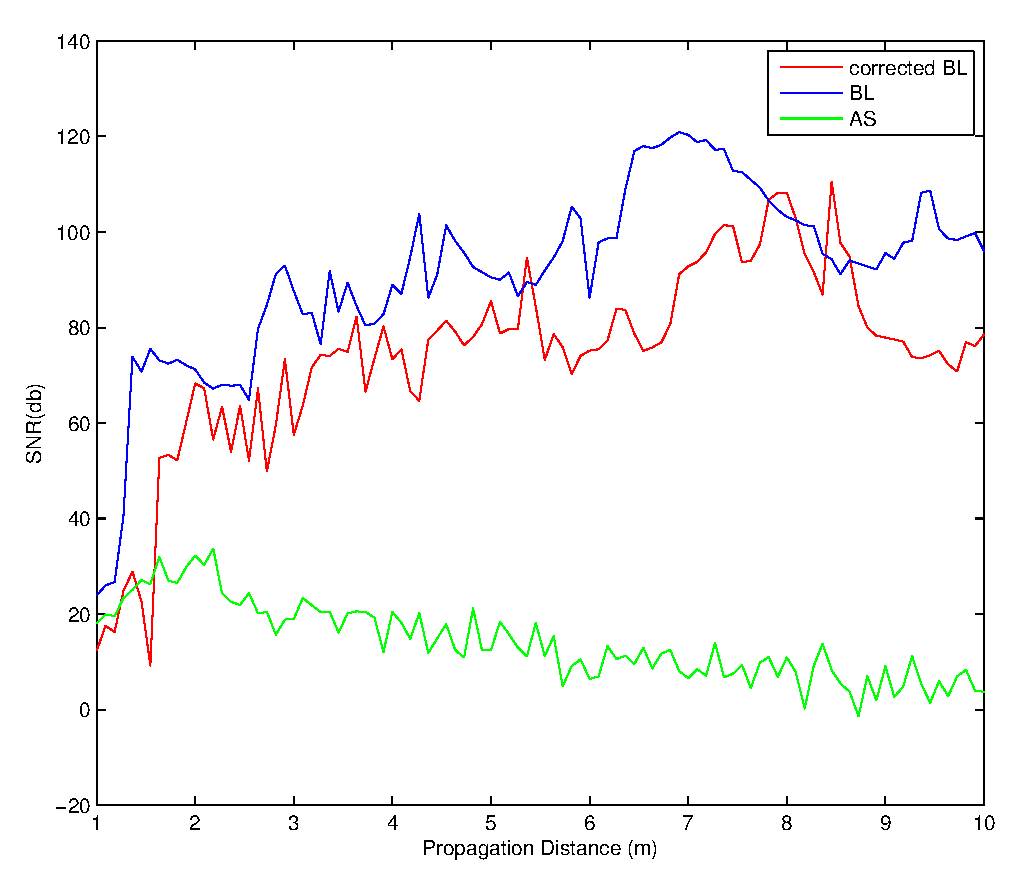
\includegraphics[height=12cm]{SNR_com.eps}
 		\end{tabular}
 	\end{center}
 	\caption	{ \label{fig:SNR1} 
 		Comparison between the Signal to Noise ratio (SNR) as a function of the propagation distance for the three propagation methods seen in section \ref{sec:angular 2}. The BL and the corrected BL methods improve the SNR, that instead drops as the propagation distance increases when the AS method is used. }
 \end{figure} 
  \begin{figure}[H]
  	\begin{center}
  		\begin{tabular}{c}
  			\includegraphics[height=15cm]{methods1.eps}
  		\end{tabular}
  	\end{center}
  	\caption{ \label{fig:methods} 
  		Comparison of the performances of the three angular spectrum propagation operator. On the left column are shown diffraction pattern cross section obtained using the angular spectrum method (AS). In the central column the pattern for the same propagation distances have been obtained using the band limited method (BL) and in the right column the same patterns have been obtained using the correct band limited method (corrected BL). }
  \end{figure}
\section{Thin Lens Operator}
\label{sec:lens}
This section will describe how the thin lens operator has been designed and implemented in the simulation toolbox, following the method described in Goodman \cite{goodman2005introduction}.
A lens is composed of a material with a refractive index different form the one of air, that causes the propagation velocity of the optical field to drop. In the approximation of a thin lens, the translation of the ray of light inside the lens is negligible and if a ray enters the lens at the coordinate $(x,y)$ on one face, it exits at the same coordinates at the other side. A thin lens delays and incident wave-front by an amount proportional to its thickness. These delay can be modelled introducing a phase factor to the incident field. 
The thickness of the lens, $\Delta(x,y)$, is a function of the coordinates \textit{(x,y)} as shown in figure \ref{fig:thick}, where $\Delta_0$ is the lens maximum thickness at the coordinates $(0,0)$.
\begin{figure}[h]
	\begin{center}
		\begin{tabular}{c}
			\includegraphics[height=5cm]{lens1.eps}
		\end{tabular}
	\end{center}
	\caption{ \label{fig:thick} 
	Thickness of a lens as a function of position along x coordinate. It can be defined in the same way along the y coordinate}
\end{figure} 
The phase delay introduced by the lens is proportional to its thickness:
\begin{equation}
\label{eq:phase}
	\phi(x,y)=kn\Delta(x,y)+k[\Delta_0-\Delta(x,y)]
\end{equation} 	
where $n$ is the refractive index of the lens material and $k=2\pi/\lambda$ is the wave number. With reference to figure \ref{fig:thick} the quantity
\begin{math}
	kn\Delta(x,y)
\end{math}
is the phase delay introduced by the different material of the lens, and 
\begin{math}
	k[\Delta_0-\Delta(x,y)]
\end{math}
is the phase delay introduced by the free space propagation between the two planes represented with dashed line.
This phase delay can be seen as a multiplicative phase term defined as:
\begin{equation}
\label{eq:delay}
	t_{lens}=\exp[jk\Delta_0]exp[jk(n-1)\Delta(x,y)]
\end{equation}
The complex field 
\begin{math}
	U'(x,y)
\end{math}
immediately after the lens is therefore given by the product of the field entering the lens 
\begin{math}
	U_0(x,y)
\end{math} 
with the phase delay in equation \ref{eq:delay}.
\begin{equation}
\label{eq:disturbance}
	U'(x,y)=t_{lens}(x,y)U_0(x,y)
\end{equation}
The sign convention used in the following derivation for a ray of light travelling form left to right is: 
\begin{itemize}
	\item any convex surface encountered has positive radius of curvature
	\item any concave surface encountered had negative radius of curvature
\end{itemize}
The lens can be split into three elements such that the total thickness function is the sum of three functions:
\begin{figure}[h]
	\begin{center}
		\begin{tabular}{c}
				\includegraphics[height=5cm]{lens2.eps}
		\end{tabular}
	\end{center}
	\caption{ \label{fig:split} 
		The thickness function can be decomposed into the sum of three contributions. }
\end{figure} 
From figure \ref{fig:split}:
\begin{equation}
\label{eq:split}
	\Delta(x,y)=\Delta_1(x,y)+\Delta_2(x,y)+\Delta_3(x,y)
\end{equation}
Where the three components of the thickness are:
\begin{equation}
\label{eq:delta1}
\Delta_1(x,y)=\Delta_{01}(x,y)-R_1\bigg(1-\sqrt{1-\frac{x^2+y^2}{R_1^2}}\bigg)
\end{equation}
\\
\begin{equation}
\label{eq:delta2}
\Delta_2(x,y)=\Delta_{02}
\end{equation}
\\
\begin{equation}
\label{eq:delta3}
\Delta_3(x,y)=\Delta_{03}(x,y)-R_2\bigg(1-\sqrt{1-\frac{x^2+y^2}{R_2^2}}\bigg)
\end{equation}
\\

\begin{math}
	R_1>0
\end{math}
and
\begin{math}
	R_2<0
\end{math}
are respectively the radius of curvature of the right-hand surface and the radius of curvature of the left-hand side of the lens surface.
Then total thickness function is given by:
\begin{equation}
\label{eq:delta_sum}
	\Delta(x,y)=\Delta_0(x,y)-R_1\bigg(1-\sqrt{1-\frac{x^2+y^2}{R_1^2}})+R_2(1-\sqrt{1-\frac{x^2+y^2}{R_2^2}}\bigg)
\end{equation}
where $\Delta_0$ is:
\begin{math}
	\Delta_0=\Delta_{01}+\Delta_{02}+\Delta_{03}
\end{math}.
In the paraxial approximation it is possible to approximate $\Delta(x,y)$ with its first element of the Taylor series:
\begin{equation}
\label{eq:approx1}
\sqrt{1-\frac{x^2+y^2}{R_1^2}}\approx 1-\frac{x^2+y^2}{R_1^2}
\end{equation}
\begin{equation}
\label{eq:approx2}
\sqrt{1-\frac{x^2+y^2}{R_2^2}}\approx 1-\frac{x^2+y^2}{R_2^2}
\end{equation}
 Substituting \ref{eq:approx1} and \ref{eq:approx2} into equation \ref{eq:delta_sum}:
 \begin{equation}
 \label{eq:approx3}
 \Delta(x,y)=\Delta_0(x,y)-\frac{x^2+y^2}{2}\bigg(\frac{1}{R_1}+\frac{1}{R_2}\bigg)
 \end{equation}
and substituting \ref{eq:approx3} into equation \ref{eq:phase} the result is the expression of the phase shift in the exponential form:
 \begin{equation}
 \label{eq:expon}
 t_{lens}(x,y)=\exp[jkn\Delta_0]exp[-jk(n-1)\frac{x^2+y^2}{2} \bigg(\frac{1}{R_1}+\frac{1}{R_2}\bigg)]
 \end{equation}
 The focal length of the lens $f$ is the quantity containing the information on the physical properties of the lens and it is defined as:
	\begin{equation}
 \label{eq:focal}
 \frac{1}{f} \equiv(n-1) \bigg(\frac{1}{R_1}+\frac{1}{R_2}\bigg)
	\end{equation}
 Finally after dropping the constant phase factor the effects of a thin lens under paraxial approximation as a quadratic phase transformation are described by equation \ref{eq:lens1}:
 \begin{equation}
 	\label{eq:lens1}
 	t_{lens}(x,y)=\exp[-j\frac{k}{2f}(x^2+y^2)]
 \end{equation}
 This equation can represent the effects of any lens, since the sign of $f$ will define whether the lens is positive or negative.
 The physical meaning of this expression can be understood through figure \ref{fig:lensmeaning}.
	\begin{figure}[h]
		\begin{center}
			\begin{tabular}{c}
					\includegraphics[height=7cm]{lens3.eps}
			\end{tabular}
		\end{center}
		\caption{ \label{fig:lensmeaning} 
			A thin lens converts a plane wave into a spherical wave. }
	\end{figure} 
	When a plane wave represented by the complex field $U(x,y)$ is normally incident on the lens, according to equation \ref{eq:disturbance}, the field leaving of the lens will be:
	\begin{equation}
	\label{eq:disturbance2}
		U'(x,y)=\exp[-j\frac{k}{2f}(x^2+y^2)]
	\end{equation}
	The thin lens is introducing a phase term on the incident field, and the resulting field is a quadratic approximation of a spherical wave. Figure \ref{fig:lensmeaning} shows that when $f$ is positive, the wave is converging towards a point on the optical axis at distance $f$ from the lens. If $f$ is negative the wave is diverging from a point on the optical axis placed at a distance $f$ in front of the lens. The lens therefore transforms a plane wave into a spherical wave. 
	The operator thin lens is defined as the product of the quadratic transformation in equation \ref{eq:lens1} with a function describing the aperture of the lens, called pupil $P(x,y)$ :
	\begin{equation}
	\label{eq:lesop}
		L(x,y)=P(x,y)\exp[-j\frac{k}{2f}(x^2+y^2)]
	\end{equation}
	where the pupil function is defined as:
	\begin{equation}
	\label{eq:pupil}
	 P(x,y) = \left\{
		\begin{array}{l l}
		1 & \quad \sqrt{x^2+y^2}<r \\
		0 & \quad \text{elsewhere}
		\end{array} \right.\
	\end{equation}
	where $r$ is the radius of the lens aperture.
	\subsection{Aliasing in Phase Sampling}
	The quadratic phase factor of the thin lens operator is a complex function whose modulus is constant and equal to unity, and its argument is an oscillating function in the interval $(0,2\pi]$. The argument of the phase factor is shown in figure \ref{fig:argument}
	\begin{figure}[H]
		\begin{center}
			\begin{tabular}{c}
					\includegraphics[height=7cm]{C:/Users/Massimo/Documents/Thesis/Thesis_PhD/figures/figurephase.png}
			\end{tabular}
		\end{center}
		\caption{ \label{fig:argument} 
			Phase profile of a computer generated lens. The blue line shows the quadratic phase term and the red line shows the same phase term wrapped every $2\pi$. This wrapping is the source of the aliasing. }
	\end{figure} 
The parabolic phase profile gets wrapped since the argument of a complex function varies between $0$ and $2\pi$. This wrapping of the phase can cause aliasing as the distance from the centre of the lens increases. For high values of $x$ and $y$, the quadratic term becomes too steep and the frequency of oscillation between $0$ and $2\pi$ of the phase factor might become too high to be correctly sampled. With analogy of what has been said in section \ref{sec:angular}, for a parabolic phase profile:
	\begin{equation}
		\label{eq:parabolic}
		\phi(x,y)=\dfrac{k}{2f}(x^2+y^2)
	\end{equation} 
The instantaneous frequencies of the phase $\nu_x$, $\nu_y$ in $x$ and $y$ respectively are defined as:
	 
\begin{equation}
\label{eq:localfreq}
\left\{
\begin{array}{l l}
\nu_x=\dfrac{1}{2\pi}\dfrac{\partial\phi}{\partial x}=\dfrac{1}{2\pi}\dfrac{k}{ f}x\\
\\
\nu_y=\dfrac{1}{2\pi}\dfrac{\partial\phi}{\partial y}=\dfrac{1}{2\pi}\dfrac{k}{ f}y
\end{array} \right.\
\end{equation}
In order to recover all the components of a periodic signal, the sampling frequency should be at least twice the bandwidth of the signal. According to the Nyquist criterion:
\begin{equation}
\label{eq:nyquist}
	f_{Nyquist}=2\nu_{max}
\end{equation} 
The maximum instantaneous frequency $\nu_{max}$ of the phase factor is the one that correspond to the edge of the lens. For brevity the one dimensional case along the $x$ direction is considered, but the conclusions are valid for the $y$ direction because of the rotational symmetry of the pupil function in equation \ref{eq:pupil}. In this case $x_{max}=y_{max}=r$ where $r$ is the radius of the pupil function.
Defining the pixel size $\Delta x$ along $x $, and assuming the pixels as square, so that the sampling frequency $1/\Delta x$ is the same along both axis, the Nyquist condition to avoid aliasing is:
\begin{equation}
	\label{eq:Nyx}
	\dfrac{1}{\Delta x}\geq \dfrac{1}{2\pi}\dfrac{k}{f}x_{max}
\end{equation}
Since in general the sampling rate cannot be modified because of the fixed pixel size of the sensor this expression leads to a condition for the radius of the pupil function:
\begin{equation}
\label{eq:radius_cond}
	r=x_{max}\leq \frac{2\pi f}{k \Delta x}
\end{equation}
Substituting $k=\frac{2\pi}{\lambda}$ into \ref{eq:radius_cond}:
\begin{equation}
\label{eq:radius_cond1}
r\leq \frac{\lambda f}{\Delta x}
\end{equation}
The more powerful the lens, $f$ will have a smaller value and hence the aperture should be smaller.
Therefore, in order to achieve a desired aperture size in equation \ref{eq:radius_cond1}, the focal length must be such that:
\begin{equation}
	\label{eq:focalcond}
	f\geq\frac{r\Delta x }{\lambda}
\end{equation}
and given that the digital resolution of a lens with aperture equal to $2r$ is given by:
\begin{equation}
\label{eq:resolution}
N=\frac{2r}{\Delta x}
\end{equation}
then the minimum resolution of a lens of radius $r$ and focal length $f$ is:
\begin{equation}
	\label{eq:rescond}
	N\geq\frac{2r^2}{f \lambda} 
\end{equation}
Applying these conditions will assure that no aliasing will be introduced by the lens operator.
 \section{Comparison between the Free Space Propagation Operators}
 \label{sec:comp}
	 In this section the differences in performance between the Fresnel approximation and the angular spectrum of plane waves approach will be shown with particular attention to the computational time required by the different methods, the optical resolution and the error. Results will be used to evaluate the characteristic of the different propagation operators. These results differ from the ones obtained in section \ref{sec:perfAS} since the simulations in this case involve the whole imaging system including the lens and not only the free space propagation.
	 \subsection{Description of the System}
	 \label{sec:system}
	 The system simulated is a simple imaging system composed of a single lens with focal length $f=158mm$, in a \textit{2f} configuration, as shown in figure \ref{fig:2f}. The field of view is a square of $1cm \times 1cm$, and the resolution of the input field is $2000 \times 2000$ pixels. The aperture of the lens is $D=5mm$ and its f number, defined as:
	 \begin{equation}
	 \label{eq:fnum}
		F_{\#}=\dfrac{z}{D}
	 \end{equation}
	 is equal to $F_{\#}=63$, where z is the distance from the lens to the image plane, that in a 2f configuration is equal to $z=2f=316mm$.
	 \begin{figure}[h]
	 	\begin{center}
	 		\begin{tabular}{c}
	 			\includegraphics[height=5cm]{C:/Users/Massimo/Documents/Thesis/Thesis_PhD/2f.eps}
	 		\end{tabular}
	 	\end{center}
	 	\caption{ \label{fig:2f} 
	 		Schematic of the 2f system simulated. f is the focal lenght, z the propagation distances, D is the aperture of the lens, w the field of view and N the sampling resolution. }
	 \end{figure} 
	 The optical cut-off frequency of this system is given by the relation \cite{goodman2005introduction}:
	 \begin{equation}
	 \label{eq:cutoff}
	 \nu_c=\dfrac{1}{\lambda F_{\#}}
	 \end{equation} 
	 The object was illuminated with monochromatic light of wavelength $\lambda=633nm$, $\nu_c=2.5\cdot10^4 cycles/m$.
	 \subsection{Image of a Point Source}
	 The first experiment simulated is the image of a point source, realized with a pinhole of $10 \mu m$ of diameter placed at the object plane indicated in figure \ref{fig:2f}. The image has been taken using four different methods to propagate the light into the system. Those are:
	 \begin{itemize}
	 	\item Multi step Fresnel method (MSF), section\ref{sec:fresnelmulti}
	 	\item Angular spectrum method (AS), section \ref{sec:angular}
	 	\item Band Limited Angular Spectrum method (BL), section \ref{sec:angular 2}
	 	\item corrected Band Limited Angular Spectrum method (CBL), section \ref{sec:angular3}
	 		 \end{itemize}
The impulse response for a point source as input will be computed using each of these methods.\\
 The sequence of operators used to simulate the system is shown in figure \ref{fig:sequence2} \\
	 \begin{figure}[H]
	 	\begin{center}
	 		\begin{tabular}{c}
	 			\includegraphics[height=1.8cm]{C:/Users/Massimo/Documents/Thesis/Thesis_PhD/imagesystem.eps}
	 		\end{tabular}
	 	\end{center}
	 	\caption{ \label{fig:sequence2} 
	 		Operator sequence for the 2f system. }
	 \end{figure} 
	 
	In the assumption of having a lens with a circular aperture and no aberrations, the impulse response of an optical system is an Airy Disk, that is the Fourier transform of the pupil of the system at the image plane. The fact that the theoretical output of the experiment is well known allows to determine the quality of the simulation tools.
	In addition to that, the Fourier transform of the impulse response of an optical system gives information on the frequencies content of the image, hence the band pass of the imaging system and its quality. 
	Figure \ref{fig:resultspoint11} shows the sensor image at the image plane together with intensity profiles of the image.
	\newpage
	 \begin{figure}[H]
	 	\begin{center}
	 		\begin{tabular}{c}
	 			\includegraphics[height=15cm]{C:/Users/Massimo/Documents/Thesis/Thesis_PhD/methodspoint1.eps}
	 		\end{tabular}
	 	\end{center}
	 	\caption{ \label{fig:resultspoint11} 
	 		From top to Bottom: Image and intensity cross section of a point source according to multi step method, angular spectrum method, band limited angular spectrum method and corrected band limited angular spectrum method. }
	 \end{figure} 
	From figure \ref{fig:resultspoint11} it can be seen that in the case of the MSF method the cross section of the impulse response does not go to zero because if additive background noise. The response of the AS method has a high frequency noise components superimposed to the diffraction pattern while the BL method reduces the noise due to aliasing of the transfer function in the AS case as can be seen comparing the two cross sections. Both the BL and the CBL methods present no background noise and in the high frequency noise is reduced with respect to the AS case. Another parameter to evaluate the accuracy of these methods is the position of the Airy disk first minimum. It is given by \cite{goodman2005introduction,pedrotti1993introduction}:
	 \begin{equation}
	 \label{eq:airy}
	 x_{min}=1.22\dfrac{\lambda z}{D}
	 \end{equation}
	 where $D$ is the aperture of the lens. According to the values in section \ref{sec:system} the Airy disk should have a its first minimum at $x_{min}=67 \mu m$.
	 Without considering the MSF case that is too noisy and does not present zeros, the position of the first minimum is the other cases are:\\
	 \begin{center}
	 \begin{tabular}{ l | r }
	 	
	 	\hline			
	 	AS & 67.5 $\mu m$ \\
	 	BL & 77.5 $\mu m$ \\
	 	CBL & 77.5 $\mu m$ \\
	 	\hline 
	 		\end{tabular}
	\end{center}
	As expected for both the band limited angular spectrum methods (BL and CBL) the Airy Disk is slightly wider due to the low pass filtering action that transfer function has undergone. However noise is reduced with the band limitation as shown in figure
	 \ref{fig:resultspoint11}.
	 To better understand how the resolution changes with the different methods, it is worth to have a look at the Fourier transform of the images shown in figure \ref{fig:resultspoint11}. The Fourier transform of the impulse response of a system give its frequency response. The shape of the frequency response gives information about how the frequency components of the input signal are modulated and transferred to the output signal. When this function goes to zero the correspondent frequency value is called the cutoff frequency. For frequencies higher than the cutoff frequency, all the information included in the input signal is lost. Results are shown in figure \ref{fig:resultspoint2}. The graphs are symmetric with respect to the zero frequency, therefore only the positive frequencies are shown.
	 
	 \begin{figure}[h]
	 	\begin{center}
	 		\begin{tabular}{c}
	 			\includegraphics[height=8cm]{C:/Users/Massimo/Documents/Thesis/Thesis_PhD/MTF.eps}
	 		\end{tabular}
	 	\end{center}
	 	\caption{ \label{fig:resultspoint2} 
	 		From top left to bottom right: Power spectrum of the image of a point source obtained with the MSF method, the AS method, the BL method and the CBL method . }
	 \end{figure} 
	From a comparison of the power spectra in figure \ref{fig:resultspoint2} it is possible to note the difference in shape of the power spectrum of the MSF method, that goes to zero slower than the angular spectrum methods spectra. These three figures present as expected the same shape since for low frequency the three angular spectrum methods are identical, with the difference of the frequency components after the cutoff frequency due to the fact that the BL and the CBL have narrower bandwidths. In the AS method graph a strong peak is present at a frequency of $10^5 m^{-1}$ due to digital artefacts arising from aliasing effects. This peak disappears in the other two band limited implementations of the angular spectrum. 
\section{Coherence}
\label{sec:coherence}
The Fresnel simulation toolbox has been designed to analyse a light field imaging system. Since all current and most future applications of plenoptic systems will have incoherently illuminated objects, the simulation of such a systems should take it into account. Therefore the decision to develop an algorithm to simulate light propagating in a low state of coherence was taken. In addition to that low coherent illumination avoids interference pattern cross talk between neighbours lenslets that might decrease the quality of the final image. \\
Coherence is a statistical property of light and is described in terms of second order averages known as coherence functions \cite{goodman2015statistical,mandel1995optical}. A full analysis of coherence of optical fields can be found in text books such as Born and Wolf \cite{born1999principles}, Mandel and Wolf \cite{mandel1995optical} and Goodman \cite{goodman2015statistical} and will not be discussed in this work. For the application described in this work coherence will be treated under a less rigorous point of view. Before analysing the computational model of coherence it is worth examining the two different types of coherence. As defined by Goodman \cite{goodman2015statistical} :
\begin{itemize}
	\item \textbf{Temporal Coherence} can be defined as the ability of light to interfere with a delayed version of itself
	\item \textbf{Spatial Coherence} can be defined as the ability of light to interfere with a spatially shifted version of itself
\end{itemize}
The empirical method developed to simulate light propagating at low coherence includes both spatial and temporal coherence. 
\subsection{Temporal Coherence}
\label{sec:temp}
Following the explanation of Goodman \cite{goodman2015statistical}, given a complex disturbance $U(\overrightarrow{X},t)$ with a finite bandwidth $\Delta\nu $, it is expected to remain constant during a time interval $\tau<1/\Delta\nu$. This means that the disturbance taken at two different times in the same spatial position $U(\overrightarrow{X},t)$ and $U(\overrightarrow{X},t+\tau)$ are highly correlated if $\tau<\tau_c$ where $\tau_c$ is the coherence time. 
Since the correlation takes place without any spatial shift it is possible to drop the spatial coordinates $\overrightarrow{X}$. The degree of temporal coherence is therefore given by the autocorrelation function:
\begin{equation}
\label{eq:coherence1}
	\Gamma(\tau) =\langle U(t+\tau)U^*(t) \rangle
\end{equation}
The coherence time $\tau$ is therefore a function of the bandwidth of the light. A perfectly monochromatic plane wave has a very narrow bandwidth and a long coherence time, while on the other hand ultra fast laser pulses will have a short coherence time and a large bandwidth. From the coherence time it is possible to define the coherence length as $l_c= v\tau_c$ where $v=c/n$ is the speed of light in the medium of propagation given by the speed of light in the vacuum $c$ divided by the refractive index $n$.
\subsection{Spatial Coherence}
To analyse spatial coherence two complex disturbances $U(\overrightarrow{X}_1,t)$ and $U(\overrightarrow{X}_2,t)$ are observed at the same time in two different position $\overrightarrow{X}_1$ and $\overrightarrow{X}_2$. When the two points coincide, $\overrightarrow{X}_1=\overrightarrow{X}_2$ the two disturbances are perfectly correlated. When the distance between the two points begins to increase, the correlation degree decreases until they become totally uncorrelated. In order to better understand this concept it is useful to illustrate the Young experiment \cite{wolf2007introduction}. With reference to figure \ref{fig:spatialcoherence} a squared light source of size $\Delta x$ emits light towards a screen at a distance R. On the screen A there are two pinholes $Q_1$ and $Q_2$. In order to have interference fringes on a second screen B the following condition should be satisfied:
\begin{equation}
\label{eq:fringes}
\Delta x \Delta \theta < \lambda
\end{equation} 
Where $2\Delta\theta$ is the angle formed at the source with the two pinholes $Q_1$ and $Q_2$ and $\lambda$ is the wavelength of the light emitted by the source. In order to see the fringes, the two pinholes should be situated in an area $\Delta A$ of size:
\begin{equation}
\label{eq:area1}
\Delta A \sim (R \Delta \theta)^2 = \dfrac{R^2}{S}\lambda
\end{equation} 
R is the distance between the screen A and the source, $S=\Delta x^2$ is the area of the source, and equation \ref{eq:fringes} has been used. The area $\Delta A$ is the coherence area of the light in the plane $A$ around the point $Q_0$ on the optical axis. 
 \begin{figure}[H]
	\centering
	\includegraphics[width=.6\textwidth]{C:/Users/Massimo/Documents/Thesis/Thesis_PhD/spatial_coherence.eps}
	\caption{\label{fig:spatialcoherence} Young experiment setup.}
\end{figure}
The area of coherence quantifies the degree of spatial coherence. It depends on the area of the light source S, the distance of observation R and the wavelength of the light. 
\subsection{Simulation of Spatial Coherence}
\label{sec:spatial}
A novel method for simulating spatial coherence that generates a source optical field with a degree of coherence defined by the user was developed and described below. An electromagnetic wave is generated by a dipole oscillating at a certain frequency. This dipole can be a molecule, an atom, a group of atoms in a gas. In case of a conventional incandescence light source light is emitted by tungsten atoms exited by the electrical current. This is also true for other sources of illuminations, like gas lamps, neon, or solid state light sources like LED; atoms of molecules excited to higher energy level emit light when dropping on the ground energy level. Each dipole emits light with a certain initial phase. Considering a light source of surface $\Sigma$ containing oscillating dipoles, the elemental surfaces $d\Sigma$ is defined as the surfaces on which all the dipoles oscillates with the same phase. The average dimension of the elemental surfaces $d\Sigma$ is proportional to the degree of spatial coherence of the light source. The more coherent the light source, the bigger the elemental surfaces will be. 
From a computational point of view having a light source composed of a mosaic of surfaces with different phases is equivalent to adding a phase mask to the input field. This phase mask is composed of areas with a random phase value. The dimension of these areas gives an idea of the degree of spatial coherence. The idea behind the empirical method used to generate the phase mask is shown in figure \ref{fig:phasemask1}: 
\begin{figure}[H]
	\begin{center}
		\begin{tabular}{c}
			\includegraphics[height=7cm]{C:/Users/Massimo/Documents/Thesis/Thesis_PhD/coherence2.eps}
		\end{tabular}
	\end{center}
	\caption{ \label{fig:phasemask1} 
		A random phase mask is generated by propagating light coming form an array of sources, each one with a random phase value in the interval $[-\pi,\pi]$. }
\end{figure} 
An array of point sources is generated on a sampling window of the same dimension as the input field. The sources are placed regularly across the array. If the number of sources is less than $20 \times 20$, the sources are displaced randomly in order not to affect the coherence with their regular structure. The square of the number of point sources used is defined as the coherence index $C$. A \textit{C} of 100 means that the initial array is composed of 100 $\times$ 100 sources. A random phase value in the range $[-\pi,\pi]$ is assigned to each of these point sources. Their amplitude is set to one. Then the array of point sources is convolved with a kernel $K$ whose size is defined in order to make all the random point sources disks of amplitude one with a finite size. All this disks touch each others without overlapping as figure \ref{fig:phasemask2} shows. The size of the kernel depends on the resolution N of the input field and on the coherence index $C$ and is equal to the ratio $N/C$.\\
The result of the convolution is a phase mask that is formed by an array of circular areas with a random phase value.
Although this array of sources is already a phase mask, it cannot be used directly in the simulation platform because of its periodicity. In fact it is not a random phase pattern. In order to randomize the shape and the distribution of the coherence areas the array of sources is propagated at a distance bigger than the size of the sources. The distance $d_c$ chosen to propagate the light sources is the one derived in section \ref{sec:fresnelmulti} to keep the same sampling both in the input and output fields using the Fresnel propagation method discussed in section. From equation \ref{eq:getz3}:
\begin{equation}
\label{eq:propcoherence}
	d_c = \dfrac{W^2}{N\lambda}
\end{equation} 
where $W$ is the field of view, $N$ is the sampling and $\lambda$ is the wavelength of the light. The choice of using the Fresnel propagation as described in section \ref{sec:Fresnel} has been made because the propagation distance is small and hence aliasing issues do not arise. In addition to that it only requires one Fourier transform, making the random phase generation algorithm faster.
The whole process is shown in figure \ref{fig:phasemask2}
\newpage
\begin{figure}[H]
	\begin{center}
		\begin{tabular}{c}
			\includegraphics[height=15cm]{C:/Users/Massimo/Documents/Thesis/Thesis_PhD/phasetarray200.eps}
		\end{tabular}
	\end{center}
	\caption	{ \label{fig:phasemask2} 
		Process of the creation of the phase mask. Top: array of point sources with a random phase value; centre: array of the areas of coherence at source after the convolution with $K$; bottom: randomized areas of coherence at object plane after the propagation of $d_c$. }
\end{figure} 
Some examples of phase masks generated from different number of sources can be seen in figure \ref{fig:phasemask3}:
\begin{figure}[H]
	\begin{center}
		\begin{tabular}{c}
			\includegraphics[height=15cm]{C:/Users/Massimo/Documents/Thesis/Thesis_PhD/phi.eps}
		\end{tabular}
	\end{center}
	\caption{ \label{fig:phasemask3} 
		Final random phase mask generated a coherence index C equals to 10, 50, 100 and 200. }
\end{figure} 
The algorithm to generate the random phase mask can be summarized as follow:
\begin{itemize}
\item A number of light sources are defined, arranged in a regular array and allocated a random phase between $-\pi$ and $\pi$. 
 \item Each source has a size diameter given by: $N/C$
 \item This array of sources is then propagated a distance $d_c$ shown in equation \ref{eq:propcoherence} in order to randomize the shape of the coherence areas.
 \item the resultant phase is used as the output phase mask to add the input field.
\end{itemize}
\newpage
\subsection{Simulation of Temporal Coherence}
\label{sec:simtempcoherence}
 As discussed in section \ref{sec:temp}, temporal coherence is defined by the time $\tau$ in which the optical wave is correlated with itself. In other words after a time $t=\tau$, the optical disturbance $U(t)$ and $U(t+\tau)$ are totally uncorrelated and cannot interfere with each other. 
To simulate this effect many snapshots of the output field are taken each time using a different random distribution of phases for the sources. Assuming that the time difference between every snapshot is larger than or equal to the coherence time $\tau$. For the application for which this toolbox has been designed it is not relevant to know the exact value of $\tau$. However, the light source used for the laboratory prototype was a Thorlabs LED Array Light Source LIU630A with a wavelength centred on 630 nm and a bandwidth $\Delta\lambda=20 nm$. The emission spectrum is shown in figure \ref{fig:emission_spectrum}.
\begin{figure}[H]
	\begin{center}
		\begin{tabular}{c}
			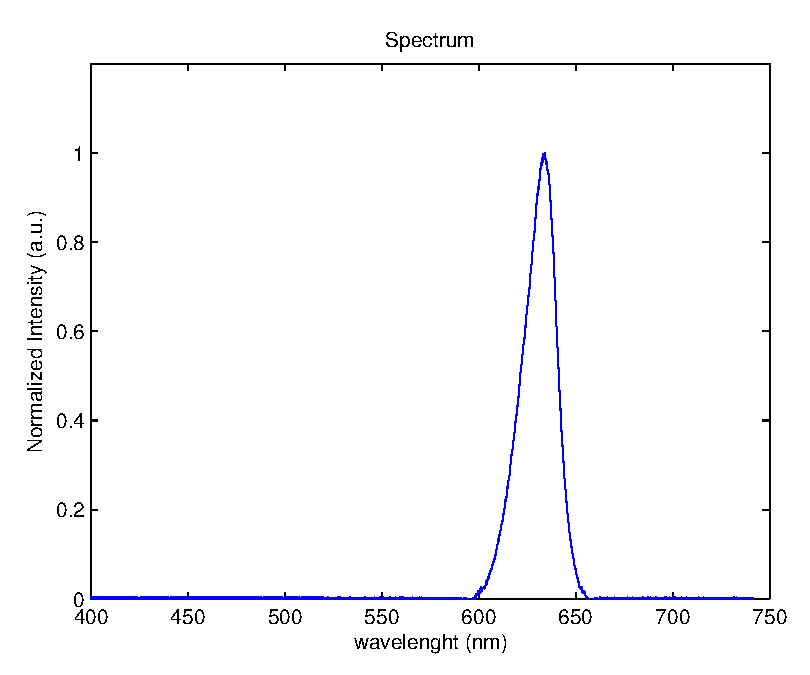
\includegraphics[height=7cm]{C:/Users/Massimo/Documents/Thesis/Thesis_PhD/spectralLED.eps}
		\end{tabular}
	\end{center}
	\caption{ \label{fig:emission_spectrum} 
		Emission spectrum of the LED considered in our simulations and real image system. Data plotted from Thorlabs LED Array Light Source LIU630A datasheet. }
\end{figure} 
 Its coherence time is given by:
\begin{equation}
\label{key}
\tau = \dfrac{1}{\Delta\nu}=\dfrac{\Delta\lambda}{c}
\end{equation}
which is equal to $\tau=6.6\times10^{-17} s$. 
 Therefore each snapshot is assumed to be taken at the image plane at an interval of $\tau$. 
 All the snapshots are then added together, integrating the optical disturbance over time. Longer integration times will give better contrast and less noise while approaching to the incoherent imaging as it is shown in the following paragraph.
 \section{Optimization of Coherence Parameters}
 The previous section described how partially coherent light is simulated and how an algorithm that produces a certain number of snapshots of the output field, each one with a different random phase, was implemented. The random phase mask simulates the spatial coherence, the number of iteration instead simulates the effects of temporal coherence.
 \subsection{Optimization of Spatial Coherence}
 Simulations have been run propagating an optical disturbance with phase masks generated with different values of the parameter \textit{C}.
 The input field is the USAF resolution target, shown in figure \ref{fig:USAF}
 \begin{figure}[H]
 	\begin{center}
 		\begin{tabular}{c}
 			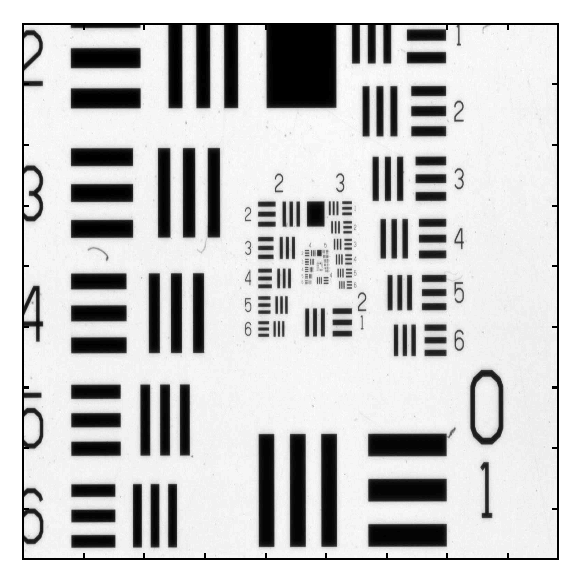
\includegraphics[height=4cm]{C:/Users/Massimo/Documents/Thesis/Thesis_PhD/USAF.eps}
 		\end{tabular}
 	\end{center}
 	\caption{ \label{fig:USAF} 
 		USAF resolution target. }
 \end{figure} 
 The first simulation has been made changing the coherence index $C$ from a value of 5 (high coherence) to 500 (low coherence) in a sampling window with a resolution of 1765 by 1765 pixels.
 Figure \ref{fig:spatialsnr2} shows how the field at the image plane for different values of \textit{C} appears, while figure \ref{fig:spatialsnr1} shows a plot of the signal to noise ratio of the images as a function of the coherence index showing an asymptotic behaviour. After a certain threshold value of $C$, increasing the coherence index does not improve the image quality. The threshold is defined as the value of $C$ for which the variance of the previous five values of SNR is less then 0.01.
Figure \ref{fig:spatialsnr1} shows that for values of $C$ bigger than 250 the SNR asymptotically tends to 18 dB. In this case the resolution of the input field, and therefore of the phase mask, is 1765 by 1765 pixels, so that the SNR reaches the asymptote when the ratio between the number of sources and the resolution is 0.14. After this point, there is no gain in making the light source more incoherent in terms of signal to noise ratio improvement.
The ratio between the number of sources \textit{C} and the resolution of the optical field \textit{N} is defined as the incoherence degree $\iota$:
\begin{equation}
\label{eq:incoherence_degree}
\iota = \dfrac{C}{N}
\end{equation}
\begin{figure}[H]
 	\centering
 	\includegraphics[width=.5\textwidth]{C:/Users/Massimo/Documents/Thesis/Thesis_PhD/iota.eps}
 	\caption{\label{fig:spatialsnr2}Images of the USAF resolution target with different values of $\iota$. Increasing the number of point sources generating the phase mask leads to more incoherent imaging, leading to improved resolution. Images where obtained with 300 iterations.}
 \end{figure}
 \begin{figure}[H]
 	\centering
 	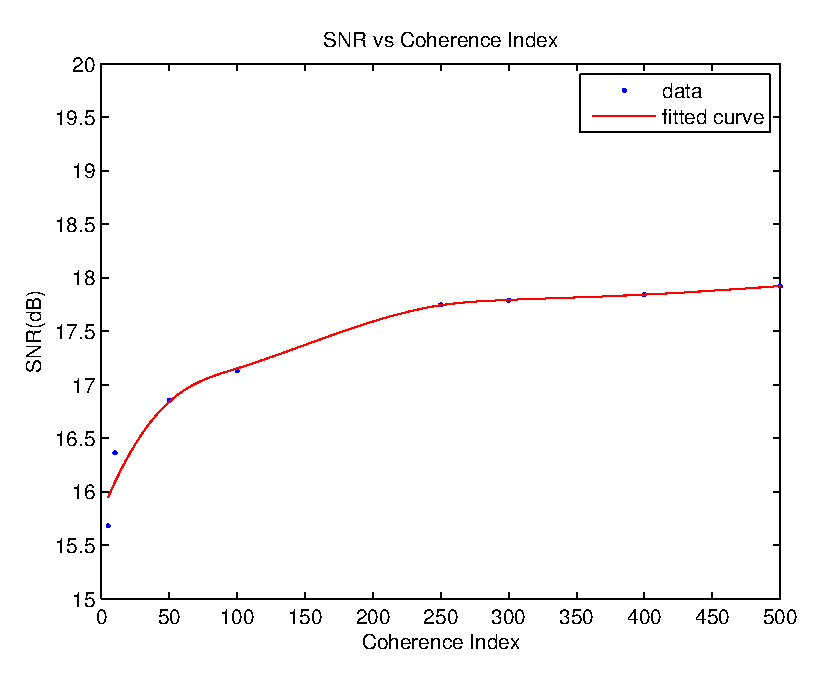
\includegraphics[width=1\textwidth]{C:/Users/Massimo/Documents/Thesis/Thesis_PhD/SNRspatial.eps}
 	\caption{\label{fig:spatialsnr1}Signal to noise ratio of the image of a USAF resolution target plotted as a function of the coherence index $C$.}
 \end{figure}
 \newpage
 \subsection{Optimization of Temporal Coherence}
The second simulation run aimed to define the optimum number of snapshots in order to correctly simulate temporal coherence. The random phase mask acts as a diffuser, and the resultant output field obtained by a single snapshot will present a low signal to noise ratio due to speckles, as shown in figure \ref{fig:speckle}
\begin{figure}[H]
	\centering
	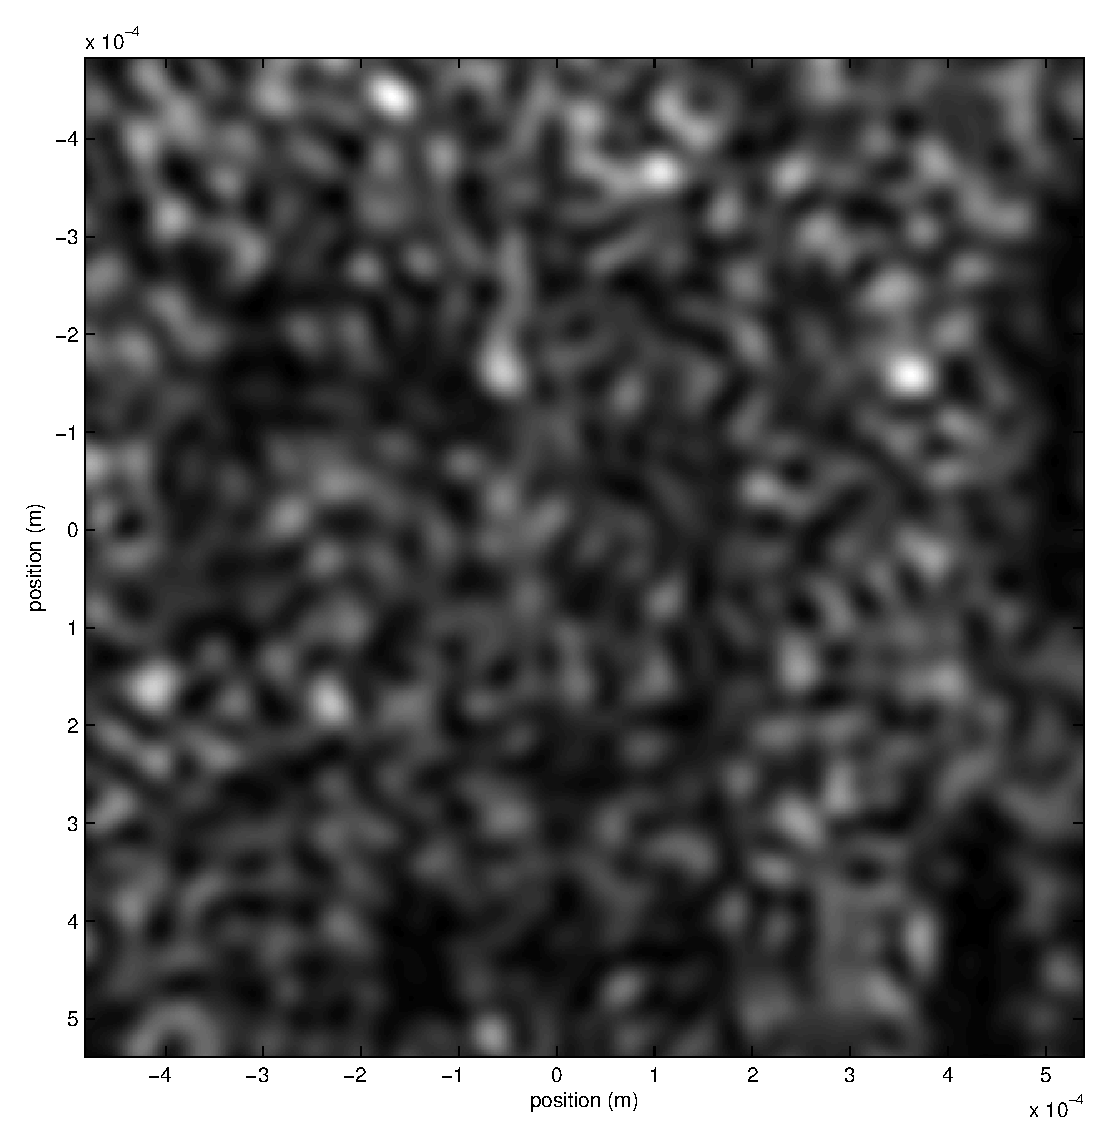
\includegraphics[width=.5\textwidth]{C:/Users/Massimo/Documents/Thesis/Thesis_PhD/USAF5iter.eps}
	\caption{\label{fig:speckle}Noise due to the speckles in an image of a USAF resolution target after only 5 iterations.}
\end{figure}
Taking several snapshots and adding them all together is equal to an integration over time of the optical field reaching the sensor. While increasing the integration time, the noise due to the speckles drops considerably. Figure \ref{fig:iter} shows several images of the USAF target in figure \ref{fig:USAF} taken with an incoherence degree of $\iota=0.14$, and with an increasing number of iterations form 5 to 1000.
 \begin{figure}[H]
 	\centering
 	\includegraphics[width=1\textwidth]{C:/Users/Massimo/Documents/Thesis/Thesis_PhD/iter.eps}
 	\caption{\label{fig:iter}Images of the USAF resolution target obtained adding an increasing number of snapshot. this is equivalent to increase the integration time of the sensor. The noise due to the speckles caused by the phase mask decreases with increasing number of iterations.}
 \end{figure}
 Since increasing the number of iterations is computationally expensive, the signal to noise ratio of the images in figure \ref{fig:iter} has been evaluated and plotted as a function of the number of iteration in order to define an optimal parameter. Results are shown in figure \ref{fig:SNRiter}. The threshold is defined as the number of iterations for which the variance of the previous five values of SNR is less then 0.01.
 \begin{figure}[H]
 	\centering
 	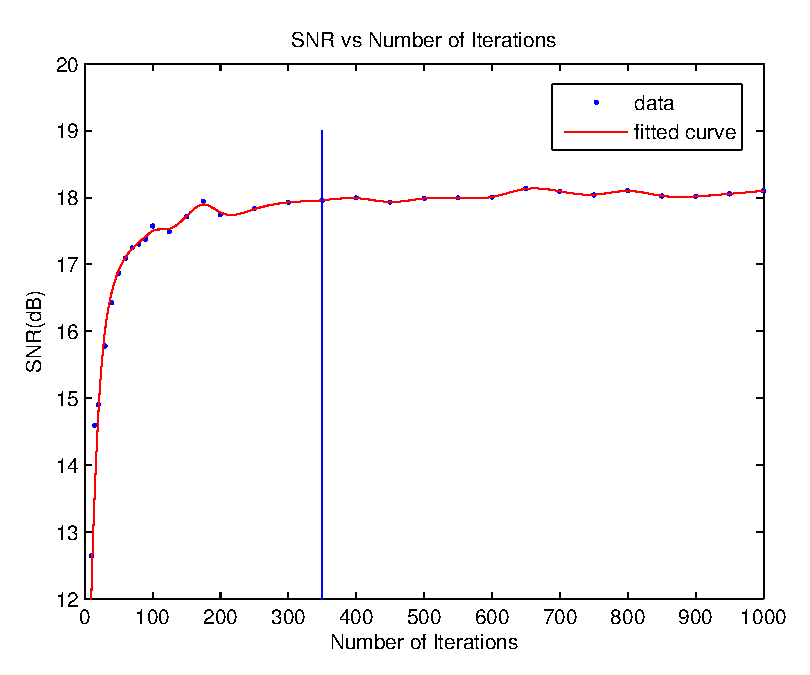
\includegraphics[width=1\textwidth]{C:/Users/Massimo/Documents/Thesis/Thesis_PhD/SNRtemporal.eps}
 	\caption{\label{fig:SNRiter}Signal to noise ratio as a function of the number of iterations. The threshold has been calculated looking at the variance of the previous five data.}
 \end{figure}
 For an image with an incoherence degree of $\iota=0.14$ the number of iterations after the SNR of the image does not improve further is 350. After that value the SNR tends asymptotically to 18 dB in spite of an increased computational effort. Therefore from a SNR point of view the optimal number of iteration to simulate temporal incoherence is 350. All the other simulations presented in this work will be performed with the coherence parameters discussed in this section. 
\subsection{Coherent Imaging vs Incoherent Imaging}
The image of an edge has been simulated to make a comparison between the coherent and the incoherent system response. Data were simulated with the same optical parameters described in section \ref{sec:system}. The intensity profile of an image of an edge is well known both in the case of coherent and incoherent illumination and provides a means of verification for the simulation methodology discussed above. Figure \ref{fig:coherenceprofile} shows the response of a coherent and an incoherent imaging systems to a sharp edge. The intensity profile of the edge is shown in green, its coherent image in blue and the incoherent image is shown in red. The coherent image presents fringes whose amplitude decreases further away form the edge. This effect is known as ringing artefacts, due to the coherent transfer function that usually presents rapid discontinuities \cite{goodman2005introduction}. Another property of the coherent image is that it crosses the actual location of the edge at 1/4 of its asymptotic value of intensity, while the incoherent image does the same at 1/2 of its asymptotic value, as can be seen in figure \ref{fig:coherenceprofile} \cite{goodman2005introduction}. Both conditions are verified by the simulations run as shown in figure \ref{fig:coherenceprofile}. \\
\\
\\
\begin{figure}[H]
	\centering
	\includegraphics[width=.9\textwidth]{C:/Users/Massimo/Documents/Thesis/Thesis_PhD/2dedge.eps}
	\caption{\label{fig:coherenceprofile}Comparison between the coherent and an incoherent response of a simple 2f system to a sharp edge.}
\end{figure}
\nomenclature{$\overrightarrow{E}$}{Electric field}
\nomenclature{$\overrightarrow{H}$}{Magnetic field}
\nomenclature{$\epsilon$}{Electrical permittivity}
\nomenclature{$\mu$}{Magnetic permittivity}
\nomenclature{$\nabla$}{Laplacian operator}
\nomenclature{$\widehat{i},\widehat{j}$, $\widehat{k}$}{unit vectors}
\nomenclature{$n$}{Refractive index}
\nomenclature{$c$}{Speed of light in vacuum}
\nomenclature{$t$}{Time}
\nomenclature{$u$}{Field disturbance}
\nomenclature{$\nu$}{Optical frequency}
\nomenclature{$\phi$}{Phase}
\nomenclature{$k$}{Wave number}
\nomenclature{$U$}{Complex field}
\nomenclature{$\eta, \chi$}{Object space coordinates}
\nomenclature{$\sigma$}{Area of the aperture}
\nomenclature{$f_x, f_y$}{Spatial frequencies}
\nomenclature{$\nu_x, \nu_y$}{Local spatial frequencies}
\nomenclature{SNR}{Signal to noise ratio}
\nomenclature{$\Delta$}{Thickness function}
\nomenclature{$t_{lens}$}{Transmission of the lens}
\nomenclature{R}{Radius of curvature of a lens surface}
\nomenclature{$N$}{Number of samples}
\nomenclature{$r$}{Radius of a lens aperture}
\nomenclature{$F_\#$}{F-number}
\nomenclature{$\nu_c$}{Optical cut-off frequency}
\nomenclature{$x_{min}$}{Position of Airy Disk first minimum}
\nomenclature{$\Gamma$}{Autocorrelation function}
\nomenclature{$\tau$}{Coherence time}
\nomenclature{$A$}{Area}
\nomenclature{$\Delta S$}{Area of the emitting source}
\nomenclature{$d\Sigma$}{Elemental area}
\nomenclature{$C$}{Coherence index}
\nomenclature{$d_c$}{Distance of propagation in the coherence algorithm}
\nomenclature{$W$}{Size of the input optical field}
\nomenclature{$\iota$}{Incoherence degree}

